\documentclass[a4paper]{scrartcl}

\usepackage[
    fancytheorems, 
    fancyproofs, 
    noindent, 
]{adam}

\usepackage{quiver}
\usepackage{mdsymbol}

\title{Geometry}
\author{Adam Kelly (\texttt{ak2316@cam.ac.uk})}
\date{\today}

\allowdisplaybreaks

\begin{document}

\maketitle 

% This is a short description of the course. It should give a little flavour of what the course is about, and what will be roughly covered in the notes.

This article constitutes my notes for the `Geometry' course, held in Lent 2022 at Cambridge. These notes are \emph{not a transcription of the lectures}, and differ significantly in quite a few areas. Still, all lectured material should be covered.



\tableofcontents

\section{Topological and Smooth Surfaces}

\subsection{Topological Surfaces}

We will begin immediately with a definition that will occupy us for some time.

\begin{definition}[Topological Surface]
    A topological surface is a topological space $\Sigma$ such that
    \begin{enumerate}[label=(\roman*)]
        \item Each $p \in \Sigma$ has an open neighbourhood $U$ with $p \in U$ such that $U$ is homeomorphic to $\R^2$, with its usual Euclidean topology.
        \item $\Sigma$ is Hausdorff and second countable.
    \end{enumerate}    
\end{definition}

Recall that a space $X$ is Hausdorff if for $p \neq q$ in $X$ there exists disjoint open sets $p \in U$ and $q \in V$ in $X$, and that a space is second countable it's topology has a countable basis.
In some ways, the real nature of topological spaces comes from the condition (a), and the condition (b) is really there for technical honesty.

\subsection{Examples of Topological Surfaces}

Let's now take some to consider some examples of topological surfaces.

\begin{example}[$\R^2$]
    The plane $\R^2$ is a topological surface.
\end{example}

\begin{example}[Subsets of $\R^2$]
    Any open subset of $\R^2$ is a topological surface. For example
    \begin{enumerate}[label=(\roman*)]
        \item $\R^2 \backslash \{0\}$ is a topological surface;
        \item Let $Z = \{(0, 0) \} \cup \{(1, 1/n) \mid n \in \N\}$, then $\R^2 \backslash Z$ is a topological surface.
    \end{enumerate}
\end{example}

\begin{example}[Graphs]
    Let $f: \R^2 \rightarrow \R$ be a continuous function. Then the \vocab{graph} 
    $$\Gamma_f = \{(x, y, f(x, y)) \mid (x, y) \in \R^2\} \subseteq \R^3 \text{ (subspace topology)}.$$
    
    Recall that if $X$ and $Y$ are topological spaces, the product topology on $X \times Y$ has basis open sets $U \times V$ with $U \subseteq X$ and $V \subseteq Y$ both open sets.

    It has the feature that $f: Z \rightarrow X \times Y$ is continuous if and only if $\pi_x \circ f: Z \rightarrow X$ and $\pi_y \circ f: Z \rightarrow Y$ are continuous.

    So if $\Gamma_f \subseteq X \times Y$ and $f: X \rightarrow Y$ is continuous then $\Gamma_f$ is homeomorphic to $X$, with the map $s: x \mapsto (x, f(x))$, so that $\left.\pi\right|_{\Gamma_f}$ and $s$ are inverse homeomorphisms.

    So $\Gamma_f \cong \R^2$ for \emph{any} continuous $f: \R^2 \rightarrow \R$, and $\Gamma_f$ is a topological surface.
\end{example}

As a note, the topological surface $\Gamma_f$ is independent of $f$. Later on as we develop more tools in geometry we will be able to better reflect the structure of the function $f$. 

\begin{example}[Stereographic Projection]
    Consider the sphere
    $$
S^2 = \{(x, y, t) \in \R^3 \mid x^2 + y^2 + z^2 =1 \}.
    $$

    We can consider the stereographic projection
    \begin{align*}
        \pi_+ : S^2 \backslash \{(0, 0, 1)\} &\rightarrow \R^2 (z = 0) \subseteq \R^3 \\
        (x, y, t) &\mapsto \left(\frac{x}{1 - t}, \frac{y}{1 - t}\right).
    \end{align*}
    Such a projection is shown below.

    \begin{center}
        

% Gradient Info
  
\tikzset {_dgh8fcybk/.code = {\pgfsetadditionalshadetransform{ \pgftransformshift{\pgfpoint{89.1 bp } { -128.7 bp }  }  \pgftransformscale{1.32 }  }}}
\pgfdeclareradialshading{_var369p8e}{\pgfpoint{-72bp}{104bp}}{rgb(0bp)=(1,1,1);
rgb(0bp)=(1,1,1);
rgb(25bp)=(0.78,0.88,1);
rgb(400bp)=(0.78,0.88,1)}
\tikzset{every picture/.style={line width=0.75pt}} %set default line width to 0.75pt        

\begin{tikzpicture}[x=0.75pt,y=0.75pt,yscale=-1,xscale=1]
%uncomment if require: \path (0,300); %set diagram left start at 0, and has height of 300

%Shape: Rectangle [id:dp9621550874774156] 
\draw   (119.66,91.2) -- (378.29,91.2) -- (330.63,158.95) -- (72,158.95) -- cycle ;
%Shape: Circle [id:dp7711674031779723] 
\path  [shading=_var369p8e,_dgh8fcybk] (168,120.2) .. controls (168,86.51) and (195.31,59.2) .. (229,59.2) .. controls (262.69,59.2) and (290,86.51) .. (290,120.2) .. controls (290,153.89) and (262.69,181.2) .. (229,181.2) .. controls (195.31,181.2) and (168,153.89) .. (168,120.2) -- cycle ; % for fading 
 \draw   (168,120.2) .. controls (168,86.51) and (195.31,59.2) .. (229,59.2) .. controls (262.69,59.2) and (290,86.51) .. (290,120.2) .. controls (290,153.89) and (262.69,181.2) .. (229,181.2) .. controls (195.31,181.2) and (168,153.89) .. (168,120.2) -- cycle ; % for border 

%Shape: Ellipse [id:dp7010564209713763] 
\draw  [dash pattern={on 0.84pt off 2.51pt}] (168,120.2) .. controls (168,110.55) and (195.31,102.74) .. (229,102.74) .. controls (262.69,102.74) and (290,110.55) .. (290,120.2) .. controls (290,129.85) and (262.69,137.66) .. (229,137.66) .. controls (195.31,137.66) and (168,129.85) .. (168,120.2) -- cycle ;
%Straight Lines [id:da601420156609989] 
\draw [color={rgb, 255:red, 74; green, 144; blue, 226 }  ,draw opacity=1 ] [dash pattern={on 4.5pt off 4.5pt}]  (229,59.2) -- (275,102.03) ;
%Shape: Circle [id:dp9581781475680486] 
\draw  [draw opacity=0][fill={rgb, 255:red, 208; green, 2; blue, 27 }  ,fill opacity=1 ] (224.75,59.2) .. controls (224.75,56.85) and (226.65,54.95) .. (229,54.95) .. controls (231.35,54.95) and (233.25,56.85) .. (233.25,59.2) .. controls (233.25,61.55) and (231.35,63.45) .. (229,63.45) .. controls (226.65,63.45) and (224.75,61.55) .. (224.75,59.2) -- cycle ;
%Straight Lines [id:da4941203681575539] 
\draw [color={rgb, 255:red, 74; green, 144; blue, 226 }  ,draw opacity=1 ]   (275,102.03) -- (322,148.45) ;
%Straight Lines [id:da7315894591096315] 
\draw [color={rgb, 255:red, 74; green, 144; blue, 226 }  ,draw opacity=1 ] [dash pattern={on 4.5pt off 4.5pt}]  (322,148.45) -- (346,172.95) ;
%Shape: Circle [id:dp7248118504557512] 
\draw  [draw opacity=0][fill={rgb, 255:red, 208; green, 2; blue, 27 }  ,fill opacity=1 ] (270.75,102.03) .. controls (270.75,99.69) and (272.65,97.78) .. (275,97.78) .. controls (277.35,97.78) and (279.25,99.69) .. (279.25,102.03) .. controls (279.25,104.38) and (277.35,106.28) .. (275,106.28) .. controls (272.65,106.28) and (270.75,104.38) .. (270.75,102.03) -- cycle ;
%Shape: Circle [id:dp13443566890481096] 
\draw  [draw opacity=0][fill={rgb, 255:red, 208; green, 2; blue, 27 }  ,fill opacity=1 ] (317.75,148.45) .. controls (317.75,146.1) and (319.65,144.2) .. (322,144.2) .. controls (324.35,144.2) and (326.25,146.1) .. (326.25,148.45) .. controls (326.25,150.8) and (324.35,152.7) .. (322,152.7) .. controls (319.65,152.7) and (317.75,150.8) .. (317.75,148.45) -- cycle ;
%Straight Lines [id:da5636421496414195] 
\draw    (72,158.95) -- (330.63,158.95) ;

% Text Node
\draw (312.6,122.5) node [anchor=north west][inner sep=0.75pt]  [color={rgb, 255:red, 208; green, 2; blue, 27 }  ,opacity=1 ]  {$\pi _{+}( p)$};
% Text Node
\draw (221.8,37.3) node [anchor=north west][inner sep=0.75pt]    {$N$};
% Text Node
\draw (254.2,88.5) node [anchor=north west][inner sep=0.75pt]    {$p$};


\end{tikzpicture}

    \end{center}

    Note that $\pi_{+}$ is continuous and has an inverse
    $$
    (u, v) \mapsto \left(\frac{2u}{u^2 + v^2 + 1}, \frac{2v}{u^2 + v^2 + 1}, \frac{u^2 + v^2 - 1}{u^2 + v^2 + 1}\right).
    $$
    So $\pi_+$ is a continuous bijection with continuous inverse and hence a homeomorphism.

    Of course we could also have projected from the south pole, to get a homeomorphism $\pi_-$ from $S^2 \backslash \{0, 0, -1\}$ to $\R^2$, so indeed every point lies in an open set which is homeomorphic through either $\pi_+$ or $\pi_-$ to $\R^2$. So $S^2$ is a topological surface.
\end{example}

\begin{remark}
    $S^2$ is compact as a topological space, since it is a closed bounded set in $\R^3$.
\end{remark}

\begin{example}[Real Projective Plane]
    The group $\Z/2\Z$ acts on $S^2$ by homeomorphisms via the \vocab{antipodal map} $a: S^2 \rightarrow S^2$ with
    $$
    a(x, y, t) = (-x, -y, -t).
    $$
    That is, there exists a homeomorphism $\Z/2\Z \rightarrow \operatorname{Homeo}(S^2)$ sending the non-identity element to $a$.

    The \vocab{real projective plane} is the quotient space of $S^2$ given by identifying every point with its antipodal image: $\R \PP^2 = S^2/(\Z/2\Z) = S^2/\sim$ with $x \sim a(x)$.

    Note that $\sim$ is the equivalence relation of belonging to the same orbit under the given action.

    As a set, $\R \PP^2$ is naturally in bijection with the set of straight lines in $\R^3$ through the origin, with the bijection given by mapping lines with the identified points on the sphere that they pass through.
    \begin{center}
        

% Gradient Info
  
\tikzset {_52kankop7/.code = {\pgfsetadditionalshadetransform{ \pgftransformshift{\pgfpoint{89.1 bp } { -128.7 bp }  }  \pgftransformscale{1.32 }  }}}
\pgfdeclareradialshading{_4ataw6yqb}{\pgfpoint{-72bp}{104bp}}{rgb(0bp)=(1,1,1);
rgb(0bp)=(1,1,1);
rgb(25bp)=(0.78,0.88,1);
rgb(400bp)=(0.78,0.88,1)}
\tikzset{every picture/.style={line width=0.75pt}} %set default line width to 0.75pt        

\begin{tikzpicture}[x=0.75pt,y=0.75pt,yscale=-1,xscale=1]
%uncomment if require: \path (0,202); %set diagram left start at 0, and has height of 202

%Shape: Circle [id:dp9158198273647966] 
\path  [shading=_4ataw6yqb,_52kankop7] (168,73) .. controls (168,39.31) and (195.31,12) .. (229,12) .. controls (262.69,12) and (290,39.31) .. (290,73) .. controls (290,106.69) and (262.69,134) .. (229,134) .. controls (195.31,134) and (168,106.69) .. (168,73) -- cycle ; % for fading 
 \draw   (168,73) .. controls (168,39.31) and (195.31,12) .. (229,12) .. controls (262.69,12) and (290,39.31) .. (290,73) .. controls (290,106.69) and (262.69,134) .. (229,134) .. controls (195.31,134) and (168,106.69) .. (168,73) -- cycle ; % for border 

%Shape: Ellipse [id:dp9820685265727336] 
\draw  [dash pattern={on 0.84pt off 2.51pt}] (168,73) .. controls (168,63.35) and (195.31,55.54) .. (229,55.54) .. controls (262.69,55.54) and (290,63.35) .. (290,73) .. controls (290,82.65) and (262.69,90.46) .. (229,90.46) .. controls (195.31,90.46) and (168,82.65) .. (168,73) -- cycle ;
%Straight Lines [id:da5819287923563754] 
\draw [color={rgb, 255:red, 74; green, 144; blue, 226 }  ,draw opacity=1 ] [dash pattern={on 4.5pt off 4.5pt}]  (177.33,93.25) -- (275,54.83) ;
%Shape: Circle [id:dp5576782083705247] 
\draw  [draw opacity=0][fill={rgb, 255:red, 208; green, 2; blue, 27 }  ,fill opacity=1 ] (224.75,73) .. controls (224.75,70.65) and (226.65,68.75) .. (229,68.75) .. controls (231.35,68.75) and (233.25,70.65) .. (233.25,73) .. controls (233.25,75.35) and (231.35,77.25) .. (229,77.25) .. controls (226.65,77.25) and (224.75,75.35) .. (224.75,73) -- cycle ;
%Straight Lines [id:da1474048195066866] 
\draw [color={rgb, 255:red, 74; green, 144; blue, 226 }  ,draw opacity=1 ]   (275,54.83) -- (372.67,16.42) ;
%Shape: Circle [id:dp7710725956210569] 
\draw  [draw opacity=0][fill={rgb, 255:red, 208; green, 2; blue, 27 }  ,fill opacity=1 ] (270.75,54.83) .. controls (270.75,52.49) and (272.65,50.58) .. (275,50.58) .. controls (277.35,50.58) and (279.25,52.49) .. (279.25,54.83) .. controls (279.25,57.18) and (277.35,59.08) .. (275,59.08) .. controls (272.65,59.08) and (270.75,57.18) .. (270.75,54.83) -- cycle ;
%Straight Lines [id:da21359057500415712] 
\draw [color={rgb, 255:red, 74; green, 144; blue, 226 }  ,draw opacity=1 ]   (79.67,131.67) -- (177.33,93.25) ;
%Shape: Circle [id:dp001468373157834657] 
\draw  [draw opacity=0][fill={rgb, 255:red, 208; green, 2; blue, 27 }  ,fill opacity=1 ] (173.08,93.25) .. controls (173.08,90.9) and (174.99,89) .. (177.33,89) .. controls (179.68,89) and (181.58,90.9) .. (181.58,93.25) .. controls (181.58,95.6) and (179.68,97.5) .. (177.33,97.5) .. controls (174.99,97.5) and (173.08,95.6) .. (173.08,93.25) -- cycle ;

% Text Node
\draw (331.67,11.57) node [anchor=north west][inner sep=0.75pt]    {$\ell $};


\end{tikzpicture}

    \end{center}

    We can also check that $\R\PP^2$ is a topological surface. 
    
    We must first check that it is Hausdorff. Recall that if $X$ is a space and $q: X \rightarrow Y$ is a quotient map, then $V \in Y$ is open if and only if $q^{-1}(V) \in X$ is open.

    \begin{center}
        

        % Gradient Info
          
        \tikzset {_xqhjp23by/.code = {\pgfsetadditionalshadetransform{ \pgftransformshift{\pgfpoint{89.1 bp } { -128.7 bp }  }  \pgftransformscale{1.32 }  }}}
        \pgfdeclareradialshading{_u4k2fy3b5}{\pgfpoint{-72bp}{104bp}}{rgb(0bp)=(1,1,1);
        rgb(0bp)=(1,1,1);
        rgb(25bp)=(0.78,0.88,1);
        rgb(400bp)=(0.78,0.88,1)}
        \tikzset{every picture/.style={line width=0.75pt}} %set default line width to 0.75pt        
        
        \begin{tikzpicture}[x=0.75pt,y=0.75pt,yscale=-1,xscale=1]
        %uncomment if require: \path (0,202); %set diagram left start at 0, and has height of 202
        
        %Shape: Circle [id:dp6622324342535655] 
        \path  [shading=_u4k2fy3b5,_xqhjp23by] (168,73) .. controls (168,39.31) and (195.31,12) .. (229,12) .. controls (262.69,12) and (290,39.31) .. (290,73) .. controls (290,106.69) and (262.69,134) .. (229,134) .. controls (195.31,134) and (168,106.69) .. (168,73) -- cycle ; % for fading 
         \draw   (168,73) .. controls (168,39.31) and (195.31,12) .. (229,12) .. controls (262.69,12) and (290,39.31) .. (290,73) .. controls (290,106.69) and (262.69,134) .. (229,134) .. controls (195.31,134) and (168,106.69) .. (168,73) -- cycle ; % for border 
        
        %Shape: Ellipse [id:dp7154492097345231] 
        \draw  [dash pattern={on 0.84pt off 2.51pt}] (168,73) .. controls (168,63.35) and (195.31,55.54) .. (229,55.54) .. controls (262.69,55.54) and (290,63.35) .. (290,73) .. controls (290,82.65) and (262.69,90.46) .. (229,90.46) .. controls (195.31,90.46) and (168,82.65) .. (168,73) -- cycle ;
        %Shape: Circle [id:dp1416961048393608] 
        \draw  [draw opacity=0][fill={rgb, 255:red, 208; green, 2; blue, 27 }  ,fill opacity=1 ] (257.15,118.2) .. controls (257.15,115.85) and (259.05,113.95) .. (261.4,113.95) .. controls (263.75,113.95) and (265.65,115.85) .. (265.65,118.2) .. controls (265.65,120.55) and (263.75,122.45) .. (261.4,122.45) .. controls (259.05,122.45) and (257.15,120.55) .. (257.15,118.2) -- cycle ;
        %Shape: Circle [id:dp6541042949762148] 
        \draw  [draw opacity=0][fill={rgb, 255:red, 208; green, 2; blue, 27 }  ,fill opacity=1 ] (264.75,37.63) .. controls (264.75,35.29) and (266.65,33.38) .. (269,33.38) .. controls (271.35,33.38) and (273.25,35.29) .. (273.25,37.63) .. controls (273.25,39.98) and (271.35,41.88) .. (269,41.88) .. controls (266.65,41.88) and (264.75,39.98) .. (264.75,37.63) -- cycle ;
        %Shape: Circle [id:dp3717908849425047] 
        \draw  [draw opacity=0][fill={rgb, 255:red, 208; green, 2; blue, 27 }  ,fill opacity=1 ] (191.08,28.05) .. controls (191.08,25.7) and (192.99,23.8) .. (195.33,23.8) .. controls (197.68,23.8) and (199.58,25.7) .. (199.58,28.05) .. controls (199.58,30.4) and (197.68,32.3) .. (195.33,32.3) .. controls (192.99,32.3) and (191.08,30.4) .. (191.08,28.05) -- cycle ;
        %Shape: Circle [id:dp48147546135749275] 
        \draw  [draw opacity=0][fill={rgb, 255:red, 208; green, 2; blue, 27 }  ,fill opacity=1 ] (187.15,114.03) .. controls (187.15,111.69) and (189.05,109.78) .. (191.4,109.78) .. controls (193.75,109.78) and (195.65,111.69) .. (195.65,114.03) .. controls (195.65,116.38) and (193.75,118.28) .. (191.4,118.28) .. controls (189.05,118.28) and (187.15,116.38) .. (187.15,114.03) -- cycle ;
        %Curve Lines [id:da617904657863573] 
        \draw [color={rgb, 255:red, 74; green, 144; blue, 226 }  ,draw opacity=1 ] [dash pattern={on 4.5pt off 4.5pt}]  (259.2,20.6) .. controls (242.8,28.6) and (256.8,67.8) .. (284.2,46.8) ;
        %Curve Lines [id:da8882017467035133] 
        \draw [color={rgb, 255:red, 74; green, 144; blue, 226 }  ,draw opacity=1 ] [dash pattern={on 4.5pt off 4.5pt}]  (178.4,106.6) .. controls (203.2,92.6) and (213,112) .. (198.8,126.2) ;
        %Curve Lines [id:da718360696826156] 
        \draw [color={rgb, 255:red, 208; green, 2; blue, 27 }  ,draw opacity=1 ] [dash pattern={on 4.5pt off 4.5pt}]  (207.2,15.8) .. controls (227.2,46.2) and (180,48.2) .. (177.2,41.8) ;
        %Curve Lines [id:da9625606480931335] 
        \draw [color={rgb, 255:red, 208; green, 2; blue, 27 }  ,draw opacity=1 ] [dash pattern={on 4.5pt off 4.5pt}]  (278.8,107.4) .. controls (256.4,91) and (233.6,125) .. (248,130.6) ;
        
        % Text Node
        \draw (280.47,23.17) node [anchor=north west][inner sep=0.75pt]    {$p$};
        % Text Node
        \draw (166.07,120.6) node [anchor=north west][inner sep=0.75pt]    {$-p$};
        % Text Node
        \draw (268.07,120.6) node [anchor=north west][inner sep=0.75pt]    {$q$};
        % Text Node
        \draw (171.67,4.6) node [anchor=north west][inner sep=0.75pt]    {$-q$};
        
        
        \end{tikzpicture}
        
            \end{center}
        

    If $[p] \neq [q] \in \R\PP^2$ then $\pm p$ and $\pm q \in S^2$ are distinct antipodal points. We can then take small open discs\footnote{We could take small balls $B_{\pm p}(\delta)$ and $B_{\pm q}(\delta)$ ($\delta \ll$ 1 small), which meet $S^2$ in open sets. If $q: S^2 \rightarrow \R\PP^2$ is the quotient map, then $q(B_{p}(\delta))$ \emph{is} open since $q^{-1}(q(B_{p}(\delta))) = B_{p}(\delta) \cup (-B_{p}(\delta))$, the union with the antipodal image.} about these in $S^2$ as in the picture, which give us disjoint open neighborhoods of $[p]$ or $[q]$ in $\R \PP^2$. That is, it's Hausdorff.

    We can also check that $\R\PP^2$ is second countable. We know that $U$ be a countable basis for the topology on $S^2$, and without loss of generality for all $u \in U$, the antipodal image is in $U$.
    Let $\overline{U}$ be the family of opens ets in $\R\PP^2$ of the form $q(u) \cup q(-u), u \in U$.
    Now if $V \subseteq \R\PP^2$ is open, by definition $q^{-1}(V)$ is open in $S^2$, and so $q^{-1}(V)$ contains some $u \in U$ and hence contains $u \cup (-u)$. So $\overline{U}$ is a countable base for the quotient topology on $\R\PP^2$.

    Finally, let $p \in S^2$ and let $[p] \in \R\PP^2$ be it's image.
    Let $\overline{D}$ be a small\footnote{Contained in an open hemisphere} closed disc neighborhood of $p \in S^2$.

    \begin{center}
        

% Gradient Info
  
\tikzset {_uh7h7p9fi/.code = {\pgfsetadditionalshadetransform{ \pgftransformshift{\pgfpoint{89.1 bp } { -128.7 bp }  }  \pgftransformscale{1.32 }  }}}
\pgfdeclareradialshading{_r893scinr}{\pgfpoint{-72bp}{104bp}}{rgb(0bp)=(1,1,1);
rgb(0bp)=(1,1,1);
rgb(25bp)=(0.78,0.88,1);
rgb(400bp)=(0.78,0.88,1)}
\tikzset{every picture/.style={line width=0.75pt}} %set default line width to 0.75pt        

\begin{tikzpicture}[x=0.75pt,y=0.75pt,yscale=-1,xscale=1]
%uncomment if require: \path (0,202); %set diagram left start at 0, and has height of 202

%Shape: Circle [id:dp6134291728044772] 
\path  [shading=_r893scinr,_uh7h7p9fi] (168,73) .. controls (168,39.31) and (195.31,12) .. (229,12) .. controls (262.69,12) and (290,39.31) .. (290,73) .. controls (290,106.69) and (262.69,134) .. (229,134) .. controls (195.31,134) and (168,106.69) .. (168,73) -- cycle ; % for fading 
 \draw   (168,73) .. controls (168,39.31) and (195.31,12) .. (229,12) .. controls (262.69,12) and (290,39.31) .. (290,73) .. controls (290,106.69) and (262.69,134) .. (229,134) .. controls (195.31,134) and (168,106.69) .. (168,73) -- cycle ; % for border 

%Shape: Ellipse [id:dp23237974780055493] 
\draw  [dash pattern={on 0.84pt off 2.51pt}] (168,73) .. controls (168,63.35) and (195.31,55.54) .. (229,55.54) .. controls (262.69,55.54) and (290,63.35) .. (290,73) .. controls (290,82.65) and (262.69,90.46) .. (229,90.46) .. controls (195.31,90.46) and (168,82.65) .. (168,73) -- cycle ;
%Shape: Circle [id:dp218060194467266] 
\draw  [draw opacity=0][fill={rgb, 255:red, 208; green, 2; blue, 27 }  ,fill opacity=1 ] (243.42,46.63) .. controls (243.42,44.29) and (245.32,42.38) .. (247.67,42.38) .. controls (250.01,42.38) and (251.92,44.29) .. (251.92,46.63) .. controls (251.92,48.98) and (250.01,50.88) .. (247.67,50.88) .. controls (245.32,50.88) and (243.42,48.98) .. (243.42,46.63) -- cycle ;
%Shape: Ellipse [id:dp6209060771777748] 
\draw  [color={rgb, 255:red, 74; green, 144; blue, 226 }  ,draw opacity=1 ] (225.71,46.63) .. controls (225.71,35.46) and (235.54,26.4) .. (247.67,26.4) .. controls (259.79,26.4) and (269.63,35.46) .. (269.63,46.63) .. controls (269.63,57.81) and (259.79,66.87) .. (247.67,66.87) .. controls (235.54,66.87) and (225.71,57.81) .. (225.71,46.63) -- cycle ;

% Text Node
\draw (254.47,33.83) node [anchor=north west][inner sep=0.75pt]    {$p$};
% Text Node
\draw (213.47,20.83) node [anchor=north west][inner sep=0.75pt]  [color={rgb, 255:red, 74; green, 144; blue, 226 }  ,opacity=1 ]  {$\overline{D}$};


\end{tikzpicture}

    \end{center}

    Then the quotient map $q|_{\overline{D}} : \overline{D} \rightarrow q(\overline{D}) \subseteq \R \PP^2$ is a continuous map from a compact space to a Hausdorff space.
    Also, on $\overline{D}$ the map $q$ is injective.
So by the topological inverse function theorem, this map $q|_{\overline{D}}$ is a homeomorphism. This induces (by taking interiors) a homeomorphism $q|_{D}: D \rightarrow q(D) \in \R\PP^2$. So $[p] \in q(D)$ has an open neighborhood in $\R\PP^2$ homeomorphic to an open disk, and we are done.

\end{example}

\begin{example}[Torus]
    Let $S^1 = \{z \in \C \mid |z| = 1\}$, and define the \vocab{torus} $S_1 \times S_1$ with the subspace topology from $\C^2$ (which is the product topology). We will show that the torus is a topological surface.

    Consider the map
    \begin{align*}
        \R^2 &\xrightarrow{\ e\ } S^1 \times S^1 \subseteq \C \times \C \\
        (s, t) & \longmapsto (e^{2\pi i s}, e^{2 \pi i t}).
    \end{align*}

    Note that this induces a map (in a set theoretic sense)
    \begin{center}
        % https://q.uiver.app/?q=WzAsMyxbMCwwLCJcXG1hdGhiYntSfV4yIl0sWzAsMiwiXFxSXjIvXFxaXjIiXSxbMiwwLCJTXjFcXHRpbWVzIFNeMSJdLFswLDFdLFswLDIsImUiXSxbMSwyLCJcXGhhdHtlfSJdXQ==
        \begin{tikzcd}[ampersand replacement=\&]
            {\mathbb{R}^2} \&\& {S^1\times S^1} \\
            \\
            {\R^2/\Z^2}
            \arrow[from=1-1, to=3-1]
            \arrow["e", from=1-1, to=1-3]
            \arrow["{\hat{e}}", from=3-1, to=1-3]
        \end{tikzcd}
    \end{center}
    that is, on the equivalence relation on $\R^2$ given by translating by $\pi^2$, $e$ is constant on equivalence classes and so induces a map of sets $\R^2/\Z^2 \rightarrow S^1 \times S^1$. Note we viewing $\R^2/\Z^2$ as the quotient space for $q: \R^2 \rightarrow \R^2/\Z^2$.

    So the map $[0, 1]^2 \hookrightarrow \R^2 \xrightarrow{q} \R^2/\Z^2$ is onto, \emph{so} $\R^2/\Z^2$ is compact. So $\hat{e}$ is a continuous map from a compact space to a Hausdorff space and is a bijection, and is thus a homeomorphism by the topological inverse function theorem.

    Note we already know that $S^1 \times S^1$ is compact and Hausdorff (closed and bounded in $\R^4$). As for $S^2 \rightarrow \R\PP^2$, pick $[p] = q(p)$ for $p \in \R^2$ and some small closed disc $\overline{D}(p) \subseteq \R^2$ such that for all non-zero integers $n, m$ we have $\overline{D}(p) \cap (\overline{D}(p) + (n, m)) = \emptyset$.
    Then $e|_{\overline{D}(p)}$ is injective and $q|_{\overline{D}(p)}$ is injective.
    Now restricting to the open disc as before, we get an open disc neighborhood of $[p] \in S^1 \times S^1$.
    Since $[p]$ is arbitrary, $S^1 \times S^1$ is a topological surface.

    Another viewpoint: $\R^2/\Z^2$ is also given by imposing on $[0, 1]^2$ the equivalence relation generated by $(x, 0) \sim (x, 1)$, $(0, y) \sim (1, y)$.
    \begin{center}
        

\tikzset{every picture/.style={line width=0.75pt}} %set default line width to 0.75pt        

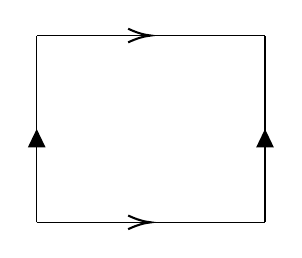
\begin{tikzpicture}[x=0.75pt,y=0.75pt,yscale=-1,xscale=1]
%uncomment if require: \path (0,202); %set diagram left start at 0, and has height of 202

%Straight Lines [id:da8677021966335143] 
\draw    (350,30) -- (460,30) ;
\draw [shift={(405,30)}, rotate = 180] [color={rgb, 255:red, 0; green, 0; blue, 0 }  ][line width=0.75]    (10.93,-3.29) .. controls (6.95,-1.4) and (3.31,-0.3) .. (0,0) .. controls (3.31,0.3) and (6.95,1.4) .. (10.93,3.29)   ;
%Straight Lines [id:da23039877923398766] 
\draw    (350,120) -- (460,120) ;
\draw [shift={(405,120)}, rotate = 180] [color={rgb, 255:red, 0; green, 0; blue, 0 }  ][line width=0.75]    (10.93,-3.29) .. controls (6.95,-1.4) and (3.31,-0.3) .. (0,0) .. controls (3.31,0.3) and (6.95,1.4) .. (10.93,3.29)   ;
%Straight Lines [id:da5789690290109974] 
\draw    (350,120) -- (350,30) ;
\draw [shift={(350,75)}, rotate = 90] [fill={rgb, 255:red, 0; green, 0; blue, 0 }  ][line width=0.08]  [draw opacity=0] (8.93,-4.29) -- (0,0) -- (8.93,4.29) -- cycle    ;
%Straight Lines [id:da42781107006682806] 
\draw    (460,120) -- (460,30) ;
\draw [shift={(460,75)}, rotate = 90] [fill={rgb, 255:red, 0; green, 0; blue, 0 }  ][line width=0.08]  [draw opacity=0] (8.93,-4.29) -- (0,0) -- (8.93,4.29) -- cycle    ;




\end{tikzpicture}

    \end{center}

\end{example}

\begin{example}[Gluing Edges]
    Let $P$ be a planar Euclidean polygon. We will assume the edges are \emph{oriented} and paired. For simplicity, we can suppose the Euclidean length of $e$ and $e'$ if $\{e, e'\}$ are paired.
    
    \begin{center}
        

\tikzset{every picture/.style={line width=0.75pt}} %set default line width to 0.75pt        

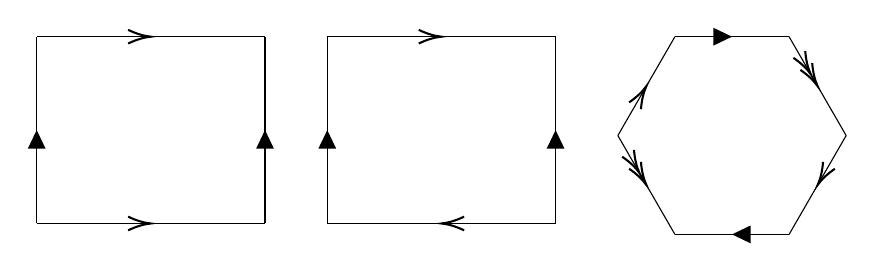
\begin{tikzpicture}[x=0.75pt,y=0.75pt,yscale=-1,xscale=1]
%uncomment if require: \path (0,202); %set diagram left start at 0, and has height of 202

%Straight Lines [id:da8677021966335143] 
\draw    (160,30) -- (270,30) ;
\draw [shift={(215,30)}, rotate = 180] [color={rgb, 255:red, 0; green, 0; blue, 0 }  ][line width=0.75]    (10.93,-3.29) .. controls (6.95,-1.4) and (3.31,-0.3) .. (0,0) .. controls (3.31,0.3) and (6.95,1.4) .. (10.93,3.29)   ;
%Straight Lines [id:da23039877923398766] 
\draw    (160,120) -- (270,120) ;
\draw [shift={(215,120)}, rotate = 180] [color={rgb, 255:red, 0; green, 0; blue, 0 }  ][line width=0.75]    (10.93,-3.29) .. controls (6.95,-1.4) and (3.31,-0.3) .. (0,0) .. controls (3.31,0.3) and (6.95,1.4) .. (10.93,3.29)   ;
%Straight Lines [id:da5789690290109974] 
\draw    (160,120) -- (160,30) ;
\draw [shift={(160,75)}, rotate = 90] [fill={rgb, 255:red, 0; green, 0; blue, 0 }  ][line width=0.08]  [draw opacity=0] (8.93,-4.29) -- (0,0) -- (8.93,4.29) -- cycle    ;
%Straight Lines [id:da42781107006682806] 
\draw    (270,120) -- (270,30) ;
\draw [shift={(270,75)}, rotate = 90] [fill={rgb, 255:red, 0; green, 0; blue, 0 }  ][line width=0.08]  [draw opacity=0] (8.93,-4.29) -- (0,0) -- (8.93,4.29) -- cycle    ;
%Straight Lines [id:da5875269260975049] 
\draw    (300,30) -- (410,30) ;
\draw [shift={(355,30)}, rotate = 180] [color={rgb, 255:red, 0; green, 0; blue, 0 }  ][line width=0.75]    (10.93,-3.29) .. controls (6.95,-1.4) and (3.31,-0.3) .. (0,0) .. controls (3.31,0.3) and (6.95,1.4) .. (10.93,3.29)   ;
%Straight Lines [id:da49746172569639246] 
\draw    (300,120) -- (410,120) ;
\draw [shift={(355,120)}, rotate = 0] [color={rgb, 255:red, 0; green, 0; blue, 0 }  ][line width=0.75]    (10.93,-3.29) .. controls (6.95,-1.4) and (3.31,-0.3) .. (0,0) .. controls (3.31,0.3) and (6.95,1.4) .. (10.93,3.29)   ;
%Straight Lines [id:da6916094237179262] 
\draw    (300,120) -- (300,30) ;
\draw [shift={(300,75)}, rotate = 90] [fill={rgb, 255:red, 0; green, 0; blue, 0 }  ][line width=0.08]  [draw opacity=0] (8.93,-4.29) -- (0,0) -- (8.93,4.29) -- cycle    ;
%Straight Lines [id:da1888172617232342] 
\draw    (410,120) -- (410,30) ;
\draw [shift={(410,75)}, rotate = 90] [fill={rgb, 255:red, 0; green, 0; blue, 0 }  ][line width=0.08]  [draw opacity=0] (8.93,-4.29) -- (0,0) -- (8.93,4.29) -- cycle    ;
%Straight Lines [id:da14721572976206643] 
\draw    (440,77.63) -- (467.5,30) ;
\draw [shift={(453.75,53.82)}, rotate = 120] [color={rgb, 255:red, 0; green, 0; blue, 0 }  ][line width=0.75]    (10.93,-3.29) .. controls (6.95,-1.4) and (3.31,-0.3) .. (0,0) .. controls (3.31,0.3) and (6.95,1.4) .. (10.93,3.29)   ;
%Straight Lines [id:da8513545957538318] 
\draw    (467.5,30) -- (522.5,30) ;
\draw [shift={(495,30)}, rotate = 180] [fill={rgb, 255:red, 0; green, 0; blue, 0 }  ][line width=0.08]  [draw opacity=0] (8.93,-4.29) -- (0,0) -- (8.93,4.29) -- cycle    ;
%Straight Lines [id:da8128090253491065] 
\draw    (522.5,30) -- (550,77.63) ;
\draw [shift={(536.25,53.82)}, rotate = 240] [color={rgb, 255:red, 0; green, 0; blue, 0 }  ][line width=0.75]    (17.64,-3.29) .. controls (13.66,-1.4) and (10.02,-0.3) .. (6.71,0) .. controls (10.02,0.3) and (13.66,1.4) .. (17.64,3.29)(10.93,-3.29) .. controls (6.95,-1.4) and (3.31,-0.3) .. (0,0) .. controls (3.31,0.3) and (6.95,1.4) .. (10.93,3.29)   ;
%Straight Lines [id:da706789823943629] 
\draw    (550,77.63) -- (522.5,125.26) ;
\draw [shift={(536.25,101.45)}, rotate = 300] [color={rgb, 255:red, 0; green, 0; blue, 0 }  ][line width=0.75]    (10.93,-3.29) .. controls (6.95,-1.4) and (3.31,-0.3) .. (0,0) .. controls (3.31,0.3) and (6.95,1.4) .. (10.93,3.29)   ;
%Straight Lines [id:da8168509195344371] 
\draw    (522.5,125.26) -- (467.5,125.26) ;
\draw [shift={(495,125.26)}, rotate = 360] [fill={rgb, 255:red, 0; green, 0; blue, 0 }  ][line width=0.08]  [draw opacity=0] (8.93,-4.29) -- (0,0) -- (8.93,4.29) -- cycle    ;
%Straight Lines [id:da057899271526199] 
\draw    (467.5,125.26) -- (440,77.63) ;
\draw [shift={(453.75,101.45)}, rotate = 240] [color={rgb, 255:red, 0; green, 0; blue, 0 }  ][line width=0.75]    (17.64,-3.29) .. controls (13.66,-1.4) and (10.02,-0.3) .. (6.71,0) .. controls (10.02,0.3) and (13.66,1.4) .. (17.64,3.29)(10.93,-3.29) .. controls (6.95,-1.4) and (3.31,-0.3) .. (0,0) .. controls (3.31,0.3) and (6.95,1.4) .. (10.93,3.29)   ;




\end{tikzpicture}

    \end{center}

    If $\{e, e'\}$ are paired edges, there is a unique isometry from $e$ to $e'$ respecting their orientations, say $f_{e e'}: e \rightarrow e'$.
    These maps generate an equivalence relation on $P$, where I identify $x \in P$ with $f_{ee'}(x)$ whenever $x \in e$. 

    \textbf{Lemma}. $P/\sim$ (with the quotient topology) is a topological surface.

    Before we prove this, we will consider the specific example of the torus as $[0, 1]^2/\sim$.

    \begin{center}
        

        \tikzset{every picture/.style={line width=0.75pt}} %set default line width to 0.75pt        
        
        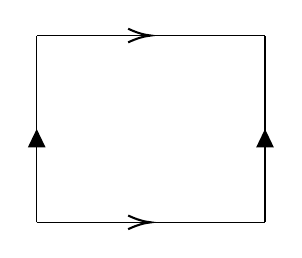
\begin{tikzpicture}[x=0.75pt,y=0.75pt,yscale=-1,xscale=1]
        %uncomment if require: \path (0,202); %set diagram left start at 0, and has height of 202
        
        %Straight Lines [id:da8677021966335143] 
        \draw    (350,30) -- (460,30) ;
        \draw [shift={(405,30)}, rotate = 180] [color={rgb, 255:red, 0; green, 0; blue, 0 }  ][line width=0.75]    (10.93,-3.29) .. controls (6.95,-1.4) and (3.31,-0.3) .. (0,0) .. controls (3.31,0.3) and (6.95,1.4) .. (10.93,3.29)   ;
        %Straight Lines [id:da23039877923398766] 
        \draw    (350,120) -- (460,120) ;
        \draw [shift={(405,120)}, rotate = 180] [color={rgb, 255:red, 0; green, 0; blue, 0 }  ][line width=0.75]    (10.93,-3.29) .. controls (6.95,-1.4) and (3.31,-0.3) .. (0,0) .. controls (3.31,0.3) and (6.95,1.4) .. (10.93,3.29)   ;
        %Straight Lines [id:da5789690290109974] 
        \draw    (350,120) -- (350,30) ;
        \draw [shift={(350,75)}, rotate = 90] [fill={rgb, 255:red, 0; green, 0; blue, 0 }  ][line width=0.08]  [draw opacity=0] (8.93,-4.29) -- (0,0) -- (8.93,4.29) -- cycle    ;
        %Straight Lines [id:da42781107006682806] 
        \draw    (460,120) -- (460,30) ;
        \draw [shift={(460,75)}, rotate = 90] [fill={rgb, 255:red, 0; green, 0; blue, 0 }  ][line width=0.08]  [draw opacity=0] (8.93,-4.29) -- (0,0) -- (8.93,4.29) -- cycle    ;
        
        
        
        
        \end{tikzpicture}
        
            \end{center}

    If $P = [0, 1]$ and $p$ is in the interior of $P$, then picking $\delta > 0$ sufficiently small so that $B_p(\delta)$ and $\overline{B_p(\delta)}$ in $\R^2$ lie in the interior of $P$. Now we argue as before: the quotient map is injective on $\overline{B_p(\delta)}$ and a homoemorphism on its interior.
    If $p$ is on an edge of $P$, then we take two half disks of sufficiently small radius $\delta$ so that they don't meet a vertex of $P$.

    \begin{center}
        


        \tikzset{every picture/.style={line width=0.75pt}} %set default line width to 0.75pt        

        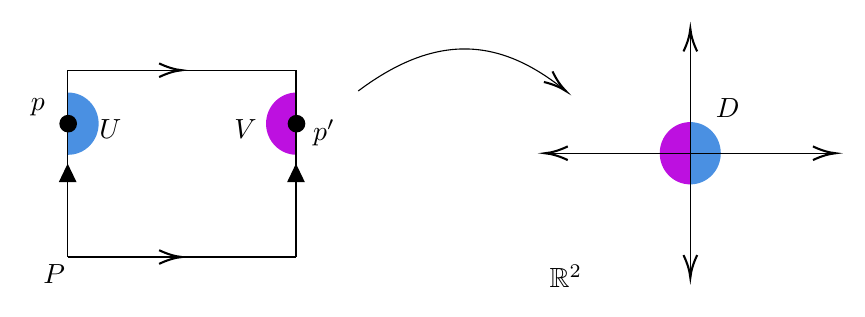
\begin{tikzpicture}[x=0.75pt,y=0.75pt,yscale=-1,xscale=1]
        %uncomment if require: \path (0,202); %set diagram left start at 0, and has height of 202
        
        %Shape: Chord [id:dp19152806356372287] 
        \draw  [draw opacity=0][fill={rgb, 255:red, 74; green, 144; blue, 226 }  ,fill opacity=1 ] (460,55) .. controls (460,55) and (460,55) .. (460,55) .. controls (460,55) and (460,55) .. (460,55) .. controls (468.1,55) and (474.67,61.72) .. (474.67,70) .. controls (474.67,78.28) and (468.1,85) .. (460,85) .. controls (459.93,85) and (459.85,85) .. (459.78,85) -- cycle ;
        %Shape: Chord [id:dp08307026163054543] 
        \draw  [draw opacity=0][fill={rgb, 255:red, 189; green, 16; blue, 224 }  ,fill opacity=1 ] (459.99,85) .. controls (459.97,85) and (459.94,85) .. (459.91,85) .. controls (451.81,85) and (445.25,78.28) .. (445.25,70) .. controls (445.25,61.72) and (451.81,55) .. (459.91,55) .. controls (459.94,55) and (459.97,55) .. (460,55) -- cycle ;
        %Shape: Chord [id:dp7404388900087537] 
        \draw  [draw opacity=0][fill={rgb, 255:red, 189; green, 16; blue, 224 }  ,fill opacity=1 ] (270.33,70.75) .. controls (270.3,70.75) and (270.28,70.75) .. (270.25,70.75) .. controls (262.15,70.75) and (255.58,64.03) .. (255.58,55.75) .. controls (255.58,47.47) and (262.15,40.75) .. (270.25,40.75) .. controls (270.28,40.75) and (270.31,40.75) .. (270.34,40.75) -- cycle ;
        %Shape: Chord [id:dp22118559447255692] 
        \draw  [draw opacity=0][fill={rgb, 255:red, 74; green, 144; blue, 226 }  ,fill opacity=1 ] (160.25,40.75) .. controls (160.25,40.75) and (160.25,40.75) .. (160.25,40.75) .. controls (160.25,40.75) and (160.25,40.75) .. (160.25,40.75) .. controls (168.35,40.75) and (174.92,47.47) .. (174.92,55.75) .. controls (174.92,64.03) and (168.35,70.75) .. (160.25,70.75) .. controls (160.18,70.75) and (160.1,70.75) .. (160.03,70.75) -- cycle ;
        %Straight Lines [id:da43490849384746944] 
        \draw    (160,30) -- (270,30) ;
        \draw [shift={(215,30)}, rotate = 180] [color={rgb, 255:red, 0; green, 0; blue, 0 }  ][line width=0.75]    (10.93,-3.29) .. controls (6.95,-1.4) and (3.31,-0.3) .. (0,0) .. controls (3.31,0.3) and (6.95,1.4) .. (10.93,3.29)   ;
        %Straight Lines [id:da02586878084495514] 
        \draw    (160,120) -- (270,120) ;
        \draw [shift={(215,120)}, rotate = 180] [color={rgb, 255:red, 0; green, 0; blue, 0 }  ][line width=0.75]    (10.93,-3.29) .. controls (6.95,-1.4) and (3.31,-0.3) .. (0,0) .. controls (3.31,0.3) and (6.95,1.4) .. (10.93,3.29)   ;
        %Straight Lines [id:da2970227178900944] 
        \draw    (160,120) -- (160,30) ;
        \draw [shift={(160,75)}, rotate = 90] [fill={rgb, 255:red, 0; green, 0; blue, 0 }  ][line width=0.08]  [draw opacity=0] (8.93,-4.29) -- (0,0) -- (8.93,4.29) -- cycle    ;
        %Straight Lines [id:da5665318796507586] 
        \draw    (270,120) -- (270,30) ;
        \draw [shift={(270,75)}, rotate = 90] [fill={rgb, 255:red, 0; green, 0; blue, 0 }  ][line width=0.08]  [draw opacity=0] (8.93,-4.29) -- (0,0) -- (8.93,4.29) -- cycle    ;
        %Shape: Circle [id:dp012642865485829713] 
        \draw  [draw opacity=0][fill={rgb, 255:red, 0; green, 0; blue, 0 }  ,fill opacity=1 ] (156,55.75) .. controls (156,53.4) and (157.9,51.5) .. (160.25,51.5) .. controls (162.6,51.5) and (164.5,53.4) .. (164.5,55.75) .. controls (164.5,58.1) and (162.6,60) .. (160.25,60) .. controls (157.9,60) and (156,58.1) .. (156,55.75) -- cycle ;
        %Shape: Circle [id:dp41106517067181514] 
        \draw  [draw opacity=0][fill={rgb, 255:red, 0; green, 0; blue, 0 }  ,fill opacity=1 ] (266,55.75) .. controls (266,53.4) and (267.9,51.5) .. (270.25,51.5) .. controls (272.6,51.5) and (274.5,53.4) .. (274.5,55.75) .. controls (274.5,58.1) and (272.6,60) .. (270.25,60) .. controls (267.9,60) and (266,58.1) .. (266,55.75) -- cycle ;
        %Curve Lines [id:da6042082411971041] 
        \draw    (300,40) .. controls (339.4,10.45) and (369.74,15.99) .. (398.68,38.94) ;
        \draw [shift={(400,40)}, rotate = 219.09] [color={rgb, 255:red, 0; green, 0; blue, 0 }  ][line width=0.75]    (10.93,-3.29) .. controls (6.95,-1.4) and (3.31,-0.3) .. (0,0) .. controls (3.31,0.3) and (6.95,1.4) .. (10.93,3.29)   ;
        %Straight Lines [id:da8873145389110244] 
        \draw    (460,12) -- (460,128) ;
        \draw [shift={(460,130)}, rotate = 270] [color={rgb, 255:red, 0; green, 0; blue, 0 }  ][line width=0.75]    (10.93,-3.29) .. controls (6.95,-1.4) and (3.31,-0.3) .. (0,0) .. controls (3.31,0.3) and (6.95,1.4) .. (10.93,3.29)   ;
        \draw [shift={(460,10)}, rotate = 90] [color={rgb, 255:red, 0; green, 0; blue, 0 }  ][line width=0.75]    (10.93,-3.29) .. controls (6.95,-1.4) and (3.31,-0.3) .. (0,0) .. controls (3.31,0.3) and (6.95,1.4) .. (10.93,3.29)   ;
        %Straight Lines [id:da20083574573053142] 
        \draw    (392,70) -- (528,70) ;
        \draw [shift={(530,70)}, rotate = 180] [color={rgb, 255:red, 0; green, 0; blue, 0 }  ][line width=0.75]    (10.93,-3.29) .. controls (6.95,-1.4) and (3.31,-0.3) .. (0,0) .. controls (3.31,0.3) and (6.95,1.4) .. (10.93,3.29)   ;
        \draw [shift={(390,70)}, rotate = 0] [color={rgb, 255:red, 0; green, 0; blue, 0 }  ][line width=0.75]    (10.93,-3.29) .. controls (6.95,-1.4) and (3.31,-0.3) .. (0,0) .. controls (3.31,0.3) and (6.95,1.4) .. (10.93,3.29)   ;
        
        % Text Node
        \draw (141,42.4) node [anchor=north west][inner sep=0.75pt]  [color={rgb, 255:red, 0; green, 0; blue, 0 }  ,opacity=1 ]  {$p$};
        % Text Node
        \draw (277,52.4) node [anchor=north west][inner sep=0.75pt]  [color={rgb, 255:red, 0; green, 0; blue, 0 }  ,opacity=1 ]  {$p'$};
        % Text Node
        \draw (147,122.4) node [anchor=north west][inner sep=0.75pt]    {$P$};
        % Text Node
        \draw (391,122.4) node [anchor=north west][inner sep=0.75pt]    {$\mathbb{R}^{2}$};
        % Text Node
        \draw (471,42.4) node [anchor=north west][inner sep=0.75pt]    {$D$};
        % Text Node
        \draw (174,52.4) node [anchor=north west][inner sep=0.75pt]    {$U$};
        % Text Node
        \draw (239,52.4) node [anchor=north west][inner sep=0.75pt]    {$V$};
        
        
        \end{tikzpicture}
        

    \end{center}

Then we can define a map $f$ from the union of these half disks to the disk of the same radius at the origin of $\R^2$ as above. 

Explicitly, we define $f_U$ and $f_V$ such that they are continuous on the half disks $U, V \in [0, 1]^2$. These induce a continuous map on $q(U)$ and $q(V) \subseteq T^2$, ($q: [0, 1]^2 \rightarrow [0, 1]^2/\sim = T^2$). In $T^2$, the half disks $q(U)$ and $q(V)$ overlap \emph{but} overlaps agree on the closed intersection locus (as $f_U$ and $f_V$ are compatible with the equivalence relation). So $f_U$ and $f_V$ glue to define a continuous map $f$ on an open neighborhood $[p] \in T^2$ to $B_0(\delta) \subseteq \R^2$.

Now we can apply our `usual argument' (pass toa closed disk, apply the topological inverse function theorem, pass back to the interior) to show that if $[q] \in R^2$ lies on the image of an edge of $[0, 1]^2$, it has an open neighborhood homeomorphic to a disk.

Analogously, at a vertex of $[0, 1]^2$, the same argument with a slight modification works.
\begin{center}
    

\tikzset{every picture/.style={line width=0.75pt}} %set default line width to 0.75pt        

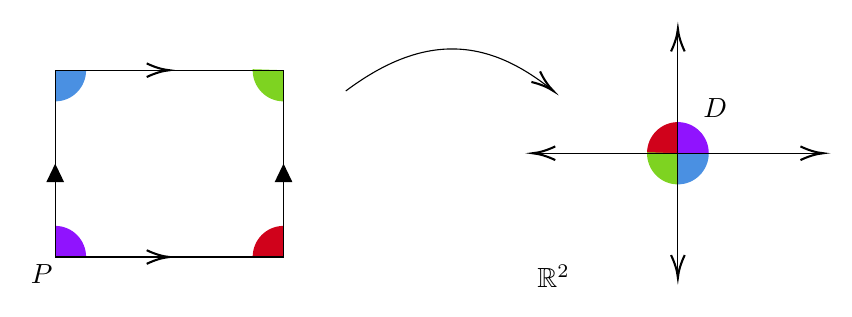
\begin{tikzpicture}[x=0.75pt,y=0.75pt,yscale=-1,xscale=1]
%uncomment if require: \path (0,202); %set diagram left start at 0, and has height of 202

%Shape: Pie [id:dp8064775069441674] 
\draw  [draw opacity=0][fill={rgb, 255:red, 74; green, 144; blue, 226 }  ,fill opacity=1 ] (474.88,70) .. controls (474.88,70) and (474.88,70) .. (474.88,70) .. controls (474.88,70) and (474.88,70) .. (474.88,70) .. controls (474.88,78.28) and (468.22,85) .. (460,85) -- (460,70) -- cycle ;
%Shape: Pie [id:dp9018456714302134] 
\draw  [draw opacity=0][fill={rgb, 255:red, 144; green, 19; blue, 254 }  ,fill opacity=1 ] (460,55) .. controls (460,55) and (460,55) .. (460,55) .. controls (468.22,55) and (474.88,61.72) .. (474.88,70) .. controls (474.88,70.03) and (474.87,70.06) .. (474.87,70.09) -- (460,70) -- cycle ;
%Shape: Pie [id:dp49066208667849565] 
\draw  [draw opacity=0][fill={rgb, 255:red, 208; green, 2; blue, 27 }  ,fill opacity=1 ] (445.13,69.87) .. controls (445.19,61.7) and (451.74,55.08) .. (459.85,55) -- (460,70) -- cycle ;
%Shape: Pie [id:dp3745820077077817] 
\draw  [draw opacity=0][fill={rgb, 255:red, 126; green, 211; blue, 33 }  ,fill opacity=1 ] (460.16,85) .. controls (460.11,85) and (460.05,85) .. (460,85) .. controls (451.78,85) and (445.13,78.28) .. (445.13,70) .. controls (445.13,69.84) and (445.13,69.68) .. (445.13,69.51) -- (460,70) -- cycle ;
%Shape: Pie [id:dp7400728219066701] 
\draw  [draw opacity=0][fill={rgb, 255:red, 74; green, 144; blue, 226 }  ,fill opacity=1 ] (174.88,30) .. controls (174.88,30) and (174.88,30) .. (174.88,30) .. controls (174.88,30) and (174.88,30) .. (174.88,30) .. controls (174.88,38.28) and (168.22,45) .. (160,45) -- (160,30) -- cycle ;
%Shape: Pie [id:dp9946660942421215] 
\draw  [draw opacity=0][fill={rgb, 255:red, 144; green, 19; blue, 254 }  ,fill opacity=1 ] (160,105) .. controls (168.22,105) and (174.88,111.72) .. (174.88,120) .. controls (174.88,120.03) and (174.87,120.06) .. (174.87,120.09) -- (160,120) -- cycle ;
%Shape: Pie [id:dp23559820712134139] 
\draw  [draw opacity=0][fill={rgb, 255:red, 208; green, 2; blue, 27 }  ,fill opacity=1 ] (255.13,119.87) .. controls (255.19,111.7) and (261.74,105.08) .. (269.85,105) -- (270,120) -- cycle ;
%Shape: Pie [id:dp44668804458299216] 
\draw  [draw opacity=0][fill={rgb, 255:red, 126; green, 211; blue, 33 }  ,fill opacity=1 ] (270.16,45) .. controls (270.11,45) and (270.05,45) .. (270,45) .. controls (261.78,45) and (255.13,38.28) .. (255.13,30) .. controls (255.13,29.84) and (255.13,29.68) .. (255.13,29.51) -- (270,30) -- cycle ;
%Straight Lines [id:da6277825936298185] 
\draw    (160,30) -- (270,30) ;
\draw [shift={(215,30)}, rotate = 180] [color={rgb, 255:red, 0; green, 0; blue, 0 }  ][line width=0.75]    (10.93,-3.29) .. controls (6.95,-1.4) and (3.31,-0.3) .. (0,0) .. controls (3.31,0.3) and (6.95,1.4) .. (10.93,3.29)   ;
%Straight Lines [id:da1928467828804079] 
\draw    (160,120) -- (270,120) ;
\draw [shift={(215,120)}, rotate = 180] [color={rgb, 255:red, 0; green, 0; blue, 0 }  ][line width=0.75]    (10.93,-3.29) .. controls (6.95,-1.4) and (3.31,-0.3) .. (0,0) .. controls (3.31,0.3) and (6.95,1.4) .. (10.93,3.29)   ;
%Straight Lines [id:da17179080567808214] 
\draw    (160,120) -- (160,30) ;
\draw [shift={(160,75)}, rotate = 90] [fill={rgb, 255:red, 0; green, 0; blue, 0 }  ][line width=0.08]  [draw opacity=0] (8.93,-4.29) -- (0,0) -- (8.93,4.29) -- cycle    ;
%Straight Lines [id:da1882407863532929] 
\draw    (270,120) -- (270,30) ;
\draw [shift={(270,75)}, rotate = 90] [fill={rgb, 255:red, 0; green, 0; blue, 0 }  ][line width=0.08]  [draw opacity=0] (8.93,-4.29) -- (0,0) -- (8.93,4.29) -- cycle    ;
%Curve Lines [id:da6787089768591394] 
\draw    (300,40) .. controls (339.4,10.45) and (369.74,15.99) .. (398.68,38.94) ;
\draw [shift={(400,40)}, rotate = 219.09] [color={rgb, 255:red, 0; green, 0; blue, 0 }  ][line width=0.75]    (10.93,-3.29) .. controls (6.95,-1.4) and (3.31,-0.3) .. (0,0) .. controls (3.31,0.3) and (6.95,1.4) .. (10.93,3.29)   ;
%Straight Lines [id:da6745216215523295] 
\draw    (460,12) -- (460,128) ;
\draw [shift={(460,130)}, rotate = 270] [color={rgb, 255:red, 0; green, 0; blue, 0 }  ][line width=0.75]    (10.93,-3.29) .. controls (6.95,-1.4) and (3.31,-0.3) .. (0,0) .. controls (3.31,0.3) and (6.95,1.4) .. (10.93,3.29)   ;
\draw [shift={(460,10)}, rotate = 90] [color={rgb, 255:red, 0; green, 0; blue, 0 }  ][line width=0.75]    (10.93,-3.29) .. controls (6.95,-1.4) and (3.31,-0.3) .. (0,0) .. controls (3.31,0.3) and (6.95,1.4) .. (10.93,3.29)   ;
%Straight Lines [id:da6300633700329288] 
\draw    (392,70) -- (528,70) ;
\draw [shift={(530,70)}, rotate = 180] [color={rgb, 255:red, 0; green, 0; blue, 0 }  ][line width=0.75]    (10.93,-3.29) .. controls (6.95,-1.4) and (3.31,-0.3) .. (0,0) .. controls (3.31,0.3) and (6.95,1.4) .. (10.93,3.29)   ;
\draw [shift={(390,70)}, rotate = 0] [color={rgb, 255:red, 0; green, 0; blue, 0 }  ][line width=0.75]    (10.93,-3.29) .. controls (6.95,-1.4) and (3.31,-0.3) .. (0,0) .. controls (3.31,0.3) and (6.95,1.4) .. (10.93,3.29)   ;

% Text Node
\draw (147,122.4) node [anchor=north west][inner sep=0.75pt]    {$P$};
% Text Node
\draw (391,122.4) node [anchor=north west][inner sep=0.75pt]    {$\mathbb{R}^{2}$};
% Text Node
\draw (471,42.4) node [anchor=north west][inner sep=0.75pt]    {$D$};


\end{tikzpicture}


\end{center}


This shows that $[0, 1]^n / \sim$ is a topological surface.

\textbf{For a general planar polygon $P$}. We will now see how to address the general case.
We again are trying to show that each point has an open neighborhood that is homeomorphic to a disk. For interior points, a suitably sizes disk (so that it does not intersect with edges or vertices).

Now we have our equivalence relation on points in the polygon $x \sim f_{ee'}(x)$ where $x \in e \in \operatorname{Edge}(P)$ and $e, e'$ are paired with $f: e \rightarrow e'$ compatible with orientation. This relation induces an equivalence relation on $\operatorname{Vert}(P)$.

If $v \in \operatorname{Vert}(p)$ has $r$ vertices in it's equivalence class, there exists $r$ sections in $P$ of total angle $\alpha_v$. Any sector can be identified with our favorite sector $(r, \theta) \in \R^2$ with $0 \leq r < \delta$ and $\theta \in [0, \alpha_v/r]$, which is homeomorphic to a disk.

To see that $P/\sim$ is Hausdorff, we can take disks on the interior with a sufficiently small radius and distinct points will have disjoint disks. For second countable, consider disks on the interior of $P$ with radional radii and center, and if $e \in \operatorname{Edge}(P)$ then $e \mapsto [0, \operatorname{length}(e)]$ is an isometry, so take only half disks on $e$ which are centered at radional radii. And at vertices, allow rational radius sectors. This gives a countable basis.


\end{example}

\begin{example}[Connect Sum]
    Given topological surfaces $\Sigma_1$ and $\Sigma_2$, we can remove an open disk from each and glue the resulting boundary circles.
    \begin{center}
        

\tikzset{every picture/.style={line width=0.75pt}} %set default line width to 0.75pt        

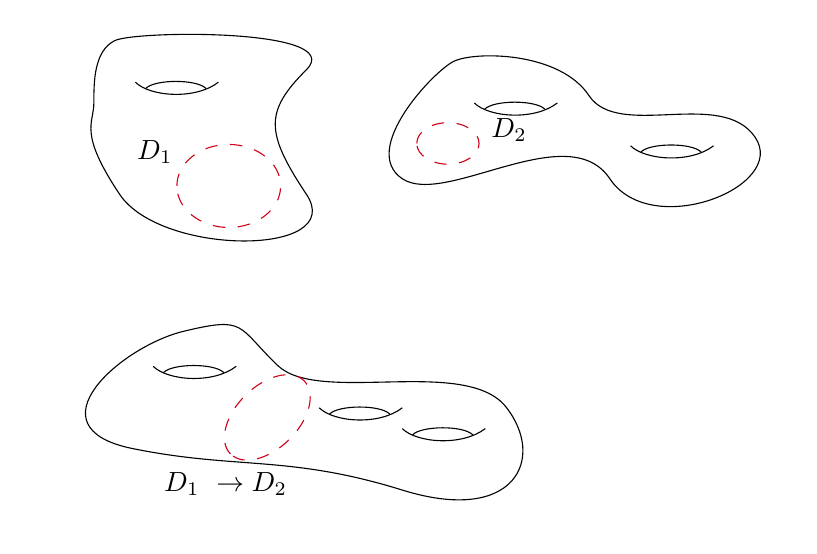
\begin{tikzpicture}[x=0.75pt,y=0.75pt,yscale=-1,xscale=1]
%uncomment if require: \path (0,264); %set diagram left start at 0, and has height of 264

%Shape: Polygon Curved [id:ds23092670908468982] 
\draw   (151.42,13.5) .. controls (161.42,8.5) and (263.82,7.5) .. (243.82,27.5) .. controls (223.82,47.5) and (223.82,57.5) .. (243.82,87.5) .. controls (263.82,117.5) and (173.82,117.5) .. (153.82,87.5) .. controls (133.82,57.5) and (141.42,53.5) .. (141.42,43.5) .. controls (141.42,33.5) and (141.42,18.5) .. (151.42,13.5) -- cycle ;
%Shape: Ellipse [id:dp8690012052686209] 
\draw  [color={rgb, 255:red, 208; green, 2; blue, 27 }  ,draw opacity=1 ][dash pattern={on 4.5pt off 4.5pt}] (181.42,83.5) .. controls (181.42,72.45) and (192.61,63.5) .. (206.42,63.5) .. controls (220.22,63.5) and (231.42,72.45) .. (231.42,83.5) .. controls (231.42,94.55) and (220.22,103.5) .. (206.42,103.5) .. controls (192.61,103.5) and (181.42,94.55) .. (181.42,83.5) -- cycle ;
%Curve Lines [id:da48090323293124504] 
\draw    (161.42,33.5) .. controls (168.42,40.5) and (190.42,42.1) .. (201.42,33.5) ;
%Curve Lines [id:da4993245884380173] 
\draw    (195.42,36.5) .. controls (190.82,31.9) and (170.62,32.1) .. (166.42,36.5) ;
%Shape: Polygon Curved [id:ds02819393118941127] 
\draw   (314.72,23.5) .. controls (324.72,18.5) and (365.8,18.6) .. (380,40) .. controls (394.2,61.4) and (443.8,36.2) .. (460,60) .. controls (476.2,83.8) and (410,110) .. (390,80) .. controls (370,50) and (310.6,93.8) .. (290,80) .. controls (269.4,66.2) and (304.72,28.5) .. (314.72,23.5) -- cycle ;
%Shape: Ellipse [id:dp20587815532253928] 
\draw  [color={rgb, 255:red, 208; green, 2; blue, 27 }  ,draw opacity=1 ][dash pattern={on 4.5pt off 4.5pt}] (297,63) .. controls (297,57.48) and (303.72,53) .. (312,53) .. controls (320.28,53) and (327,57.48) .. (327,63) .. controls (327,68.52) and (320.28,73) .. (312,73) .. controls (303.72,73) and (297,68.52) .. (297,63) -- cycle ;
%Curve Lines [id:da6703282110854694] 
\draw    (324.72,43.5) .. controls (331.72,50.5) and (353.72,52.1) .. (364.72,43.5) ;
%Curve Lines [id:da9543971323835057] 
\draw    (358.72,46.5) .. controls (354.12,41.9) and (333.92,42.1) .. (329.72,46.5) ;
%Curve Lines [id:da9854855073902014] 
\draw    (400,64.13) .. controls (407,71.13) and (429,72.73) .. (440,64.13) ;
%Curve Lines [id:da34286221876508605] 
\draw    (434,67.13) .. controls (429.4,62.53) and (409.2,62.73) .. (405,67.13) ;
%Shape: Polygon Curved [id:ds42009985613789946] 
\draw   (184.72,153.5) .. controls (215,146.2) and (210.2,151) .. (230,170) .. controls (249.8,189) and (320.6,165.4) .. (340,190) .. controls (359.4,214.6) and (344.6,247) .. (290,230) .. controls (235.4,213) and (210.2,220.2) .. (160,210) .. controls (109.8,199.8) and (154.44,160.8) .. (184.72,153.5) -- cycle ;
%Curve Lines [id:da7043527326865702] 
\draw    (170,170.38) .. controls (177,177.38) and (199,178.98) .. (210,170.38) ;
%Curve Lines [id:da06585957049626234] 
\draw    (204,173.38) .. controls (199.4,168.78) and (179.2,168.98) .. (175,173.38) ;
%Curve Lines [id:da29024936577184723] 
\draw    (250,190.38) .. controls (257,197.38) and (279,198.98) .. (290,190.38) ;
%Curve Lines [id:da781291913898559] 
\draw    (284,193.38) .. controls (279.4,188.78) and (259.2,188.98) .. (255,193.38) ;
%Curve Lines [id:da017965701892596053] 
\draw    (290,200.38) .. controls (297,207.38) and (319,208.98) .. (330,200.38) ;
%Curve Lines [id:da9180721180833686] 
\draw    (324,203.38) .. controls (319.4,198.78) and (299.2,198.98) .. (295,203.38) ;
%Shape: Ellipse [id:dp8566081737085667] 
\draw  [color={rgb, 255:red, 208; green, 2; blue, 27 }  ,draw opacity=1 ][dash pattern={on 4.5pt off 4.5pt}] (207.23,212.59) .. controls (201.4,206.7) and (204.63,194.05) .. (214.45,184.34) .. controls (224.26,174.63) and (236.94,171.52) .. (242.77,177.41) .. controls (248.6,183.3) and (245.37,195.95) .. (235.55,205.66) .. controls (225.74,215.37) and (213.06,218.48) .. (207.23,212.59) -- cycle ;

% Text Node
\draw (161,60.4) node [anchor=north west][inner sep=0.75pt]    {$D _{1}$};
% Text Node
\draw (331.72,49.9) node [anchor=north west][inner sep=0.75pt]    {$D _{2}$};
% Text Node
\draw (286.6,104.96) node [anchor=north west][inner sep=0.75pt]  [font=\Large,rotate=-89.92]  {$\longrightsquigarrow $};
% Text Node
\draw (174,220.4) node [anchor=north west][inner sep=0.75pt]    {$D _{1} \ \rightarrow D _{2}$};


\end{tikzpicture}

    \end{center}

Explicitly, I take $\Sigma_1 \backslash D_1$ and $\Sigma_2 \backslash D_2$ and impose an equivalence relation
$$
\theta \in D_1 \sim \theta \in D_2,
$$
where $\theta$ parameterises $S_1 = \delta D_i$.

The result $\Sigma_1 \# \Sigma_2$ is the \vocab{connect sum} of $\Sigma_1$ and $\Sigma_2$. Note that in principle this connect sum depends on a number of choices, but we suppress this from the notation.

Indeed, the connect sum of topological surfaces is a topological surface. This is proved as before.
\end{example}


% It is not to hard to think up many exotic 'surfaces' with different characteristics: holes, no holes, bounded, unbounded, and so on.

% \begin{center}
    

% \tikzset{every picture/.style={line width=0.75pt}} %set default line width to 0.75pt        

% \begin{tikzpicture}[x=0.75pt,y=0.75pt,yscale=-1,xscale=1]
% %uncomment if require: \path (0,300); %set diagram left start at 0, and has height of 300

% %Shape: Circle [id:dp591684684256957] 
% \draw   (60,110) .. controls (60,87.91) and (77.91,70) .. (100,70) .. controls (122.09,70) and (140,87.91) .. (140,110) .. controls (140,132.09) and (122.09,150) .. (100,150) .. controls (77.91,150) and (60,132.09) .. (60,110) -- cycle ;
% %Shape: Ellipse [id:dp6271436208495527] 
% \draw  [dash pattern={on 4.5pt off 4.5pt}] (60,110) .. controls (60,104.48) and (77.91,100) .. (100,100) .. controls (122.09,100) and (140,104.48) .. (140,110) .. controls (140,115.52) and (122.09,120) .. (100,120) .. controls (77.91,120) and (60,115.52) .. (60,110) -- cycle ;
% %Shape: Polygon Curved [id:ds2919643672856125] 
% \draw   (169.85,112.46) .. controls (170.85,81.46) and (200.85,102.32) .. (219.85,102.46) .. controls (238.85,102.6) and (272.56,83.74) .. (269.85,112.46) .. controls (267.13,141.17) and (235.99,120.6) .. (219.85,122.46) .. controls (203.7,124.32) and (168.85,143.46) .. (169.85,112.46) -- cycle ;
% %Curve Lines [id:da29495862583968235] 
% \draw    (178.85,110.46) .. controls (187.18,118.79) and (203.18,116.13) .. (208.85,110.46) ;
% %Curve Lines [id:da05574670652938796] 
% \draw    (183.85,113.46) .. controls (190.56,108.74) and (198.56,109.6) .. (203.85,113.46) ;
% %Curve Lines [id:da9130401683536076] 
% \draw    (230.85,109.68) .. controls (239.18,118.01) and (255.18,115.35) .. (260.85,109.68) ;
% %Curve Lines [id:da7204510994314768] 
% \draw    (235.85,112.68) .. controls (242.56,107.97) and (250.56,108.82) .. (255.85,112.68) ;
% %Curve Lines [id:da2773823088001599] 
% \draw    (300,70) .. controls (319.67,91) and (319.67,130.33) .. (300,150) ;
% %Curve Lines [id:da9640418131331623] 
% \draw    (354,70) .. controls (335,90.33) and (335.67,130.33) .. (354,150) ;
% %Shape: Ellipse [id:dp22219783359667034] 
% \draw  [dash pattern={on 4.5pt off 4.5pt}] (315,110) .. controls (315,107.24) and (320.6,105) .. (327.5,105) .. controls (334.4,105) and (340,107.24) .. (340,110) .. controls (340,112.76) and (334.4,115) .. (327.5,115) .. controls (320.6,115) and (315,112.76) .. (315,110) -- cycle ;
% %Straight Lines [id:da16456755952599722] 
% \draw  [dash pattern={on 0.84pt off 2.51pt}]  (354,70) -- (362,61) ;
% %Straight Lines [id:da7546245438033814] 
% \draw  [dash pattern={on 0.84pt off 2.51pt}]  (300,70) -- (293,63) ;
% %Straight Lines [id:da9016788212880511] 
% \draw  [dash pattern={on 0.84pt off 2.51pt}]  (300,150) -- (294,156) ;
% %Straight Lines [id:da09916176203257931] 
% \draw  [dash pattern={on 0.84pt off 2.51pt}]  (354,150) -- (360,156) ;
% %Straight Lines [id:da28760276070953084] 
% \draw    (410,100) -- (510,100) ;
% %Straight Lines [id:da6331102333453389] 
% \draw  [dash pattern={on 0.84pt off 2.51pt}]  (510,100) -- (530,100) ;
% %Straight Lines [id:da21402696096677087] 
% \draw  [dash pattern={on 0.84pt off 2.51pt}]  (390,100) -- (410,100) ;
% %Straight Lines [id:da1318444055095227] 
% \draw    (410,130) -- (510,130) ;
% %Straight Lines [id:da3814972937738479] 
% \draw  [dash pattern={on 0.84pt off 2.51pt}]  (510,130) -- (530,130) ;
% %Straight Lines [id:da5990977106686659] 
% \draw  [dash pattern={on 0.84pt off 2.51pt}]  (390,130) -- (410,130) ;
% %Curve Lines [id:da8167058041805688] 
% \draw    (420,112.22) .. controls (425.56,120.56) and (436.22,117.89) .. (440,112.22) ;
% %Curve Lines [id:da07278542081013839] 
% \draw    (423.33,115.22) .. controls (427.81,110.51) and (433.14,111.37) .. (436.67,115.22) ;
% %Curve Lines [id:da23375889947741713] 
% \draw    (448,112.22) .. controls (453.56,120.56) and (464.22,117.89) .. (468,112.22) ;
% %Curve Lines [id:da8125417949179057] 
% \draw    (451.33,115.22) .. controls (455.81,110.51) and (461.14,111.37) .. (464.67,115.22) ;
% %Curve Lines [id:da989215927108835] 
% \draw    (475,111.7) .. controls (480.56,120.04) and (491.22,117.37) .. (495,111.7) ;
% %Curve Lines [id:da7272978688417131] 
% \draw    (478.33,114.7) .. controls (482.81,109.99) and (488.14,110.85) .. (491.67,114.7) ;
% %Straight Lines [id:da2512282339351666] 
% \draw  [dash pattern={on 0.84pt off 2.51pt}]  (505,114) -- (525,114) ;
% %Straight Lines [id:da05590955730268288] 
% \draw  [dash pattern={on 0.84pt off 2.51pt}]  (392,114) -- (412,114) ;




% \end{tikzpicture}

% \end{center}

% In this course we will frequently deal with such surfaces, and they are studied through the lense of topological surfaces.





% We care a significant amount about $X$ random object.

% \begin{definition}[Random Object]
%     We say that an object $X$ is a \vocab{random object} if we literally do not care about what it actually is.
% \end{definition}

% It is trivial to check that all objects you will meet in this course are random objects.


\end{document}
